\documentclass[UTF8]{ctexart}
\usepackage{ctex}
\usepackage{geometry}
\usepackage{enumitem}
\usepackage{indentfirst}
\usepackage{color}
\usepackage{fancyhdr}
\usepackage{amsmath}
\usepackage{graphicx}
\usepackage{amssymb}
\usepackage{tikz}
\usepackage{cases}
\usepackage{array}
\usepackage{pgfplots}
\usepackage{tkz-euclide}

% 设置纸张和页边距——A4
\geometry{papersize={21cm,29.7cm}}
\geometry{left=3.18cm,right=3.18cm,top=2.54cm,bottom=2.54cm}

% 一级标题靠左
\CTEXsetup[format={\Large\bfseries}]{section}

% 去除页眉
\pagestyle{plain}

%设置段间距
\addtolength{\parskip}{.4em}
%%设置行间距
%\usepackage{setspace}
%\setstretch{2.5}

% 开始文档内容
\begin{document}

\title{信号与系统课程笔记:Lecture 9}
\author{授课教师:秦雨潇 \\
        笔记记录:李梦薇}
\date{2023 年 10 月 20 日(第七周,周五)}
\maketitle

\section{复习}

\subsection{信号的分解}
$f(t)=\sum_{i=k}^{l}C_iv_i(t)$\quad$a,b\in\mathbb{R}$\quad$a<b$\quad$\{v_i(t)\}$为正交完备集 \par
其中,$C_i=\frac{\langle{f(t),v_i(t)}\rangle}{\langle{v_i(t),v_i(t)}\rangle}
=\frac{1}{\|v_i(t)\Vert^2}\int_{a}^{b}f(t)v_i(t){\rm{dt}}$ \par

\subsection{Fourier Series 的三角形式}
$f(t)=\frac{a_0}{2}+\sum_{n=1}^{+\infty}[a_n\cos(\frac{2\pi}{T}nt)+b_n\sin(\frac{2\pi}{T}nt)]$\quad$t\in[0,T]$ \par
其中,$a_n=\frac{2}{T}\int_{0}^{T}f(t)\cos(\frac{2\pi}{T}nt){\rm{dt}}$

\subsection{Fourier Series 的余弦形式}
$f(t)=\frac{a_0}{2}+\sum_{n=1}^{+\infty}[A_n\cos(\frac{2\pi}{T}nt-\psi_n)]=A_0+\sum_{n=1}^{+\infty}[A_n\cos(\frac{2\pi}{T}nt-\psi_n)]$ \par
其中,$A_n=\sqrt{{a_n}^2+{b_n}^2}$\quad$\psi=\arctan(\frac{b_n}{a_n})$

\section{傅里叶级数(Fourier Series,FS)的指数(exp)形式}
\subsection{数学理解}
$e^{j\psi}=\cos{\psi}+j\sin(\psi)$
\begin{center}
    \begin{tikzpicture}
        \begin{axis}[
            width=8cm, height=8cm,
            axis lines=center,
            axis line style={->}, % 去掉箭头
            xlabel={$\text{Re}$},
            ylabel={$\text{Im}$},
            xmin=-1.3, xmax=1.3,
            ymin=-1.3, ymax=1.3,
            xtick={-1,0,1},
            ytick={-1,0,1},
            xticklabels={-1,0,1},
            yticklabels={-1,0,1},
            legend style={at={(1,1)},anchor=north west}
        ]
    
        % 绘制欧拉公式
        \draw (axis cs:0,0) circle [radius=1];
        \addplot[color=blue, domain=0:360, samples=360,smooth] ({cos(x)},{sin(x)});
        \legend{$e^{i\psi}$}

        % 添加角度为\psi的箭头、标签等
        \draw[->] (axis cs:0,0) -- (axis cs:0.707,0.707);
        \node[anchor=east] at (axis cs:0,0.707) {$j\sin(\psi)$};
        \node[anchor=north] at (axis cs:0.707,0) {$\cos(\psi)$};
        \draw[dashed] (axis cs:0.707,0) -- (axis cs:0.707,0.707);
        \draw[dashed] (axis cs:0,0.707) -- (axis cs:0.707,0.707);
        \node[anchor=north] at (axis cs:0.2,0.2) {$\psi$};
        \end{axis}
    \end{tikzpicture}
\end{center} \par

$\cos(\psi)=\frac{1}{2}(e^{j\psi}+e^{-j\psi})$
\begin{center}
    \begin{tikzpicture}
        \begin{axis}[
            width=8cm, height=8cm,
            axis lines=center,
            axis line style={->}, % 去掉箭头
            xlabel={$\text{Re}$},
            ylabel={$\text{Im}$},
            xmin=-1.3, xmax=1.3,
            ymin=-1.3, ymax=1.3,
            xtick={-1,0,1},
            ytick={-1,0,1},
            xticklabels={-1,0,1},
            yticklabels={-1,0,1},
            legend style={at={(1,1)},anchor=north west}
        ]
    
        % 计算 \cos(\psi) 的实部和虚部
        \addplot[color=blue, domain=0:360, samples=360,smooth] ({0.5*(cos(x) + cos(-x))},{0.5*(sin(x) + sin(-x))});
        \addlegendentry{$\cos(\psi)$};

        % \psi
        \draw[->] (axis cs:0,0) -- (axis cs:0.707,0.707);
        \draw[dashed] (axis cs:0.707,0) -- (axis cs:0.707,0.707);
        \draw[dashed] (axis cs:0,0.707) -- (axis cs:0.707,0.707);
        \node[anchor=north] at (axis cs:0.25,0.25) {$\psi$};
        \node[anchor=north] at (axis cs:0.9,0.9) {$e^{j\psi}$};
        % -\psi
        \draw[->] (axis cs:0,0) -- (axis cs:0.707,-0.707);
        \draw[dashed] (axis cs:0.707,0) -- (axis cs:0.707,-0.707);
        \draw[dashed] (axis cs:0,-0.707) -- (axis cs:0.707,-0.707);
        \node[anchor=south] at (axis cs:0.25,-0.25) {$-\psi$};
        \node[anchor=south] at (axis cs:0.9,-0.9) {$e^{-j\psi}$};
        % \frac{1}{2}(e^{j\psi}+e^{-j\psi})
        \draw[->,color=red] (axis cs:0,0) -- (axis cs:1,0);
        \addlegendimage{color=red, thick};
        \addlegendentry{$\frac{1}{2}(e^{j\psi}+e^{-j\psi})$};
        \end{axis}
    \end{tikzpicture}
\end{center} \par

$\sin(\psi)=\frac{1}{2j}(e^{j\psi}-e^{-j\psi})$
\begin{center}
    \begin{tikzpicture}
        \begin{axis}[
            width=8cm, height=8cm,
            axis lines=center,
            axis line style={->}, % 去掉箭头
            xlabel={$\text{Re}$},
            ylabel={$\text{Im}$},
            xmin=-1.3, xmax=1.3,
            ymin=-1.3, ymax=1.3,
            xtick={-1,0,1},
            ytick={-1,0,1},
            xticklabels={-1,0,1},
            yticklabels={-1,0,1},
            legend style={at={(1,1)},anchor=north west}
        ]
    
        % 计算 j\sin(\psi) 的实部和虚部
        \addplot[color=blue, domain=0:360, samples=360,smooth] ({0.5*(cos(x) - cos(-x))},{0.5*(sin(x) - sin(-x))});
        \addlegendentry{$j\sin(\psi)$};
        
        % \psi
        \draw[->] (axis cs:0,0) -- (axis cs:0.707,0.707);
        \draw[dashed] (axis cs:0.707,0) -- (axis cs:0.707,0.707);
        \draw[dashed] (axis cs:0,0.707) -- (axis cs:0.707,0.707);
        \node[anchor=north] at (axis cs:0.25,0.25) {$\psi$};
        \node[anchor=north] at (axis cs:0.9,0.9) {$e^{j\psi}$};
        % -\psi
        \draw[->] (axis cs:0,0) -- (axis cs:0.707,-0.707);
        \draw[dashed] (axis cs:0.707,0) -- (axis cs:0.707,-0.707);
        \draw[dashed] (axis cs:0,-0.707) -- (axis cs:0.707,-0.707);
        \node[anchor=south] at (axis cs:0.25,-0.25) {$-\psi$};
        \node[anchor=south] at (axis cs:0.9,-0.9) {$e^{-j\psi}$};
        % \frac{1}{2}(e^{j\psi}-e^{-j\psi})
        \draw[->,color=red] (axis cs:0,0) -- (axis cs:0,1);
        \addlegendimage{color=red, thick};
        \addlegendentry{$\frac{1}{2}(e^{j\psi}-e^{-j\psi})$};
        \end{axis}
    \end{tikzpicture}
\end{center} \par
\textbf{推导:}
\begin{flalign*}
    \hspace*{2em}f(t)&=\frac{A_0}{2}+\sum_{n=1}^{+\infty}\frac{A_n}{2}[e^{j(\frac{2\pi}{T}nt+\psi_n)}+e^{-j(\frac{2\pi}{T}nt+\psi_n)}]\qquad\rightarrow\frac{2\pi}{T}=\Omega &\\
    \hspace*{2em}&=\frac{A_0}{2}+\sum_{n=1}^{+\infty}\frac{A_n}{2}[e^{j\Omega{nt}}e^{j\psi_n}+e^{-j\Omega{nt}}e^{-j\psi_n}] &\\
    \hspace*{2em}&=\frac{A_0}{2}+\sum_{n=1}^{+\infty}\frac{A_n}{2}e^{j\Omega{nt}}e^{j\psi_n}+\sum_{n=-1}^{-\infty}\frac{A_n}{2}e^{j\Omega{nt}}e^{j\psi_n}\qquad\rightarrow{A_n}\text{和}\psi_n\text{的}n\text{仅表示序号,与正负无关} &\\
    \hspace*{2em}&=\frac{A_0}{2}+\sum_{n=-\infty,n\neq0}^{+\infty}\frac{A_n}{2}e^{j\Omega{nt}}e^{j\psi_n} &\\
    \hspace*{2em}&=\sum_{n=-\infty}^{+\infty}\frac{A_n}{2}e^{j\psi_n}e^{j\Omega{nt}} &\\
    \hspace*{2em}&=\sum_{n=-\infty}^{+\infty}\frac{A_n}{2}e^{j\psi_n}e^{j\frac{2\pi}{T}nt}
\end{flalign*} \par
令$F_n=\frac{A_n}{2}e^{j\psi_n}$,则$f(t)=\sum_{n=-\infty}^{+\infty}F_ne^{j\frac{2\pi}{T}nt}\quad\rightarrow{\quad}e^{j\frac{2\pi}{T}nt}=v_i(t)$?那么$e^{j\frac{2\pi}{T}nt}$是否为正交完备集?\par
\textbf{证明:}
\begin{enumerate}[label=(\arabic*),itemindent=0pt,labelindent=\parindent,labelwidth=2em,labelsep=5pt,leftmargin=*]
    \item $e^{jkx},e^{jlx}\quad{x\in[0,2\pi]\quad{k,l\in\mathbb{Z}}}$是否正交?\par
          \begin{flalign*}
            \int_{0}^{2\pi}e^{jkx}e^{-jlx}{\rm{dx}}&=\int_{0}^{2\pi}e^{j(k-l)x}e{\rm{dx}} &\\
            &=\left\{
            \begin{aligned}
                &k=l\quad\int_{0}^{2\pi}{\rm{dx}}=2\pi \\
                &k\neq{l}\quad\frac{1}{k-l}e^{j(k-l)x}\big|_{0}^{2\pi}=0
            \end{aligned}
            \right.
          \end{flalign*} \par
          由此可见正交,等同于$e^{j\frac{2\pi}{T}kx},e^{j\frac{2\pi}{T}lx}\quad{x\in[0,T]}$正交。
    \item 完备(详见书籍等证明资料)。
\end{enumerate} \par
因此,$e^{j\frac{2\pi}{T}nt}$是正交完备集。那么,$F_n=C_i=\frac{\langle{f(t),e^{j\Omega{nt}}}\rangle}{\|e^{j\Omega{nt}}\Vert^2}=\frac{1}{T}\int_{0}^{T}f(t)e^{-j\Omega{nt}}{\rm{dt}}$。\par
\textbf{综上所述,FS 的指数形式为:}\par
$f(t)=\sum_{n=-\infty}^{+\infty}F_ne^{jn\Omega{t}}$,其中$F_n=\frac{1}{T}\int_{0}^{T}f(t)e^{-jn\Omega{t}}{\rm{dt}}\qquad\rightarrow\omega=n\Omega$ \par
或$f(t)=\sum_{n=-\infty}^{+\infty}F_n(\omega)e^{j\omega{t}}$,其中$F_n(\omega)=\frac{1}{T}\int_{0}^{T}f(t)e^{-j\omega{t}}{\rm{dt}}$ \par

\subsection{几何理解}
$f(t_0)=3e^{j1\Omega{t_0}}+2e^{j2\Omega{t_0}}+1e^{j3\Omega{t_0}}$ \par
\begin{center}
    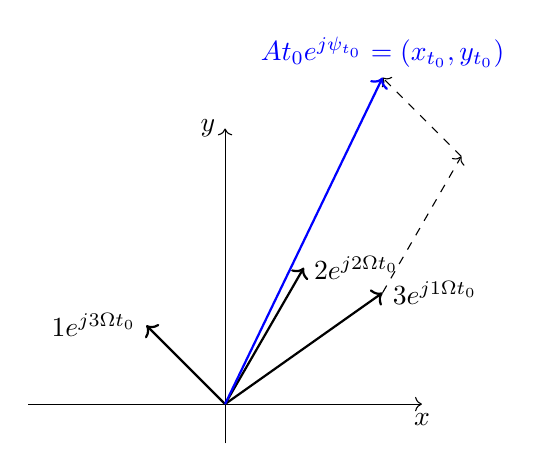
\begin{tikzpicture}
        % 绘制 x 和 y 轴
        \draw[->] (-2.5, 0) -- (2.5, 0) node[below] {$x$};
        \draw[->] (0, -0.5) -- (0, 3.5) node[left] {$y$};
        
        % 绘制向量1
        \draw[->, thick] (0, 0) -- (2, 1.414) node[right] {$3e^{j1\Omega{t_0}}$};
        
        % 绘制向量2
        \draw[->, thick] (0, 0) -- (1, 1.732) node[right] {$2e^{j2\Omega{t_0}}$};
        
        % 绘制向量3
        \draw[->, thick] (0, 0) -- (-1, 1) node[left] {$1e^{j3\Omega{t_0}}$};
        
        % 绘制向量相加的过程(虚线表示)
        \draw[->, dashed] (2, 1.414) -- (3, 3.146);
        \draw[->, dashed] (3, 3.146) -- (2, 4.146);
        \draw[->, thick, blue] (0, 0) -- (2, 4.146) node[anchor=south] {$At_0e^{j\psi_{t_0}}=(x_{t_0},y_{t_0})$};
    \end{tikzpicture}
\end{center} \par
$f(t)$“一般”情况下是实数信号时,
$f(t)=\sum_{n=-\infty}^{+\infty}F_ne^{jn\Omega{t}}$,
则$F_n=F_{-n}$,$F[n,\Omega]=F[-n,\Omega]$,$n\Omega{t}=-n\Omega{t}$($\psi_n=\psi_{-n}$)。
由此可知,我们只需要记录$F_n$一半的信号。

\section{几种特殊形式函数的 FS}
\begin{enumerate}[label=(\arabic*),itemindent=0pt,labelindent=\parindent,labelwidth=2em,labelsep=5pt,leftmargin=*]
    \item 偶函数:$b_i=0$
    \item 奇函数:$a_0=0\quad a_i=0$
    \item 奇谐函数:半波镜像\par
          \begin{center}
            \begin{tikzpicture}
            \begin{axis}[
                    width=10cm, height=6cm,
                    axis lines=center,
                    xtick={0, pi/2, pi, 3*pi/2, 2*pi},
                    xticklabels={0, $\frac{T}{2}$, $T$, $\frac{3T}{2}$, $2T$},
                    ytick=\empty,
                    xmin=-0.2, xmax=2*pi+0.5,
                    ymin=-1.2, ymax=1.2,
                ]
                \addplot[blue, domain=0:{pi/2}, samples=100, smooth] {1};
                \addplot[blue, domain={pi/2}:pi, samples=100, smooth] {-1};
                \addplot[blue, domain=pi:{3*pi/2}, samples=100, smooth] {1};
                \addplot[blue, domain={3*pi/2}:{2*pi}, samples=100, smooth] {-1};
                \draw[dashed] (axis cs:{pi/2}, -1) -- (axis cs:{pi/2}, 1);
                \draw[dashed] (axis cs:pi, -1) -- (axis cs:pi, 1);
                \draw[dashed] (axis cs:{3*pi/2}, -1) -- (axis cs:{3*pi/2}, 1);
                \draw[dashed] (axis cs:2*pi, -1) -- (axis cs:2*pi, 0);
            \end{axis}
            \end{tikzpicture}
          \end{center}
    \item 偶谐函数:半波重叠\par
          \begin{center}
            \begin{center}
                \begin{tikzpicture}
                    \begin{axis}[
                        width=10cm, height=6cm,
                        axis lines=center,
                        xtick={0, pi/2, pi, 3*pi/2, 2*pi},
                        xticklabels={0, $\frac{T}{2}$, $T$, $\frac{3T}{2}$, $2T$},
                        ytick=\empty,
                        xmin=-0.2, xmax=2*pi+0.5,
                        ymin=-1.2, ymax=1.2,
                    ]
                    \addplot[blue, domain=0:2*pi, samples=400, smooth] {abs(sin(2*deg(x))}; % 绘制 |cos(x)| 的图形
                \end{axis}
                \end{tikzpicture}
              \end{center}
          \end{center}
\end{enumerate} \par

\section{频谱}
\begin{enumerate}[label=(\arabic*),itemindent=0pt,labelindent=\parindent,labelwidth=2em,labelsep=5pt,leftmargin=*]
    \item $F_n=\frac{A_n}{2}e^{j\psi_n}\quad{[-\pi,\pi]}\quad\rightarrow\quad|F_n|=\frac{A_n}{2}$ \par
          \begin{center}
          \begin{tikzpicture}
            \begin{axis}[
                width=11cm, height=6cm,
                axis lines=center,
                xlabel={$n/n\Omega/\omega$},
                x label style={at={(ticklabel* cs:1)}, anchor=west},
                xmin=-6.5, xmax=6.5,
                ymin=0, ymax=2.5,
                xtick={-6, -5, -4, -3, -2, -1, 0, 1, 2, 3, 4, 5, 6},
                ytick=\empty,
                y axis line style={draw=none},
                legend style={at={(1.1,1)}, anchor=north west},
            ]
            \addplot[blue, mark=*, only marks] coordinates {
                (-6, 2)
                (-5, 0.5)
                (-4, 0.7)
                (-3, 0.9)
                (-2, 1.1)
                (-1, 1.3)
                (0, 1.5)
                (1, 1.3)
                (2, 1.1)
                (3, 0.9)
                (4, 0.7)
                (5, 0.5)
                (6, 2)
            };
            \legend{$F_n$};
            \draw[dashed] (axis cs:-6, 2) -- (axis cs:-6, -0.1);
            \draw[dashed] (axis cs:-5, 0.5) -- (axis cs:-5, -0.1);
            \draw[dashed] (axis cs:-4, 0.7) -- (axis cs:-4, -0.1);
            \draw[dashed] (axis cs:-3, 0.9) -- (axis cs:-3, -0.1);
            \draw[dashed] (axis cs:-2, 1.1) -- (axis cs:-2, -0.1);
            \draw[dashed] (axis cs:-1, 1.3) -- (axis cs:-1, -0.1);
            \draw[dashed] (axis cs:0, 1.5) -- (axis cs:0, -0.1);
            \draw[dashed] (axis cs:1, 1.3) -- (axis cs:1, -0.1);
            \draw[dashed] (axis cs:2, 1.1) -- (axis cs:2, -0.1);
            \draw[dashed] (axis cs:3, 0.9) -- (axis cs:3, -0.1);
            \draw[dashed] (axis cs:4, 0.7) -- (axis cs:4, -0.1);
            \draw[dashed] (axis cs:5, 0.5) -- (axis cs:5, -0.1);
            \draw[dashed] (axis cs:6, 2) -- (axis cs:6, -0.1);
            \node[anchor=south] at (axis cs:-6,2) {$F_{-6}$};
            \node[anchor=south] at (axis cs:0,1.5) {$F_0$};
            \node[anchor=south] at (axis cs:1,1.3) {$F_{1}$};
            \node[anchor=south] at (axis cs:6,2) {$F_{6}$};
            \end{axis}
          \end{tikzpicture}
          \end{center} \par
    \item $\sum{F_ne^{j\omega{t}}}=\sum{|F_n|e^{j\psi_n}e^{j\omega{t}}}$ \par
          $\psi_1=-\psi_{-1}\quad\psi_2=-\psi_{-2}\quad\psi_3=-\psi_{-3}\quad\ldots\quad\psi_n=-\psi_{-n}$
          \begin{center}
          \begin{tikzpicture}
            \begin{axis}[
                width=7cm, height=7cm,
                axis lines=center,
                x label style={at={(ticklabel* cs:1)}, anchor=west},
                xmin=-3.5, xmax=3.5,
                ymin=-2, ymax=2,
                xtick={-3, -2, -1, 0, 1, 2, 3},
                ytick=\empty,
                y axis line style={draw=none},
                legend style={at={(1.1,1)}, anchor=north west},
            ]
            \addplot[blue, mark=*, only marks] coordinates {
                (-3, -1.5)
                (-2, -0.5)
                (-1, -1)
                (1, 1)
                (2, 0.5)
                (3, 1.5)
            };
            \legend{$\psi_n$};
            \draw[dashed] (axis cs:-3, -1.5) -- (axis cs:-3, 0);
            \draw[dashed] (axis cs:-2, -0.5) -- (axis cs:-2, 0);
            \draw[dashed] (axis cs:-1, -1) -- (axis cs:-1, 0);
            \draw[dashed] (axis cs:1, 1) -- (axis cs:1, 0);
            \draw[dashed] (axis cs:2, 0.5) -- (axis cs:2, 0);
            \draw[dashed] (axis cs:3, 1.5) -- (axis cs:3, 0);
            \node[anchor=north] at (axis cs:-3, -1.5) {$\psi_{-3}$};
            \node[anchor=north] at (axis cs:-2, -0.5) {$\psi_{-2}$};
            \node[anchor=north] at (axis cs:-1, -1) {$\psi_{-1}$};
            \node[anchor=south] at (axis cs:1, 1) {$\psi_1$};
            \node[anchor=south] at (axis cs:2, 0.5) {$\psi_2$};
            \node[anchor=south] at (axis cs:3, 1.5) {$\psi_3$};
            \end{axis}
          \end{tikzpicture}
          \end{center} \par
          注意:实数情况下才成立。
\end{enumerate}

\end{document}